\newpage
\NewsItem{Luftfeuchtigkeitsmessung mittels Tauspiegelverfahren}
\begin{multicols}{3}
%%======================================================================== Text Einfügen
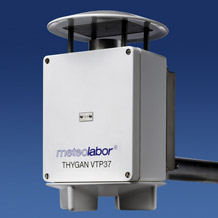
\includegraphics[width=0.3\textwidth]{graphics/thygan.jpg}
Das von der MeteoSchweiz benutzte Gerät Thygan nutzt das Taupunktspiegelverfahren, um die Luftfeuchtigkeit zu messen.\\
Dieses Verfahren beruht auf der physikalischen Beziehung zwischen Wasserdampfgehalt und Kondensationstemperatur des Wasserdampfes in einem Gasgemisch. Ein Spiegel wird abgekühlt bis mit einem optischen Element Kondensat detektiert wird. Das optische Element registriert die Reflexionsverhältnisse des Spiegels, womit dieser auf die Taupunkttemperatur eingeregelt wird. Die Taupunkttemperatur ist erreicht wenn die Temperatur des Spiegels diese unterschreitet und dadurch beschlägt, womit die Reflexion beeinträchtigt wird. Die Temperatur des Spiegels wird mit einem Temperaturfühler gemessen, dazu muss dieser sich direkt am Spiegel befinden. Mit dieser Taupunkttemperatur wird dann über eine Kennlinie der Wert der Luftfeuchtigkeit ermittelt.

\end{multicols} 
